In Chapter~\ref{ch:pes-statistics}, we saw that the photoemission statistics are influenced by the characteristics of the light source, that exhibit well-defined statistical properties. Understanding these specific characteristics can be helpful in designing tailored, model-based denoisers. For Poisson noise, we employed the Anscombe transform combined with \gls{BM3D} (\cref{sec:poisson-noise-model}). While the Anscombe transform is capable of stabilizing Poisson-distributed noise into approximately Gaussian noise for moderate to high counts, it is less effective for very low counts ($<3$), where the approximation breaks down. Similarly, a \gls{VST} tailored for \gls{NB} statistics in conjunction with \gls{BM3D} could be more effective to reduce noise.

Model-based approaches such as these can be powerful but assume that the noise characteristics are accurately known and that the underlying signal conforms to the priors encoded. However, \gls{FEL}-based photoemission experiments involve complex and heterogeneous noise sources. Factors such as long-term fluctuations in \gls{FEL} intensity (\cref{section:fel-stats}), advanced detector designs (\cref{section:8s-dld}) and environmental variations can lead to deviations from idealized models like Poisson or \gls{NB} noise prior. Adapting model-based methods to account for these complexities requires significant effort and may still fall short when dealing with unknown or dynamically changing noise patterns.

Unlike model-based methods, which depend on predefined assumptions about the noise and other image priors, machine and deep learning methods can learn these relationships directly from data. This data-driven approach allows deep learning models to handle diverse and complex noise distributions, including those that are non-standard, multi-modal, or vary across a dataset. Furthermore, \gls{CNN}-based architectures excel at extracting non-linear and hierarchical features from such high-dimensional data, structures typical of \gls{MPES} datasets. This allows to take advantage of the spatial and temporal correlations across multiple dimensions more effectively than many traditional approaches.

Machine learning can be broadly categorized in two categories: the \textit{supervised} and the \textit{unsupervised} setting. In supervised learning, the experience (\textit{model}) is learned by exposure to data containing information additional (labeled data) to what the model is supposed to map. The exposure to such data, called \textit{training}, enables the model to establish a relationship between the inputs and their corresponding outputs. The model’s expertise can then be used to map new inputs to their corresponding outputs. In the context of image restoration, the model can gain expertise from pairs of corrupted and clean images, and then use this expertise to restore other corrupted images.

Conversely, in the unsupervised setting, the model is exposed to the data without any labeled information, and the model is supposed to learn the underlying structure of the data. In context of image restoration, that would imply only giving the model the corrupted images, and expecting to map to the desired target--the clean image.

This chapter, we will discuss the foundations of learning, covering the elements of how and why learning works. This is general to both the supervised and unsupervised setting. There the concepts of \textit{hypothesis class}, \textit{capacity}, \textit{realizability}, and the concept of \textit{generalization} capability are discussed. Then we take a look at a statistical learning\footnote{Machine learning and statistical learning are many times used interchangeably but the latter places more emphasis on the statistical properties of the learning algorithms, and the former on the algorithmic aspects.} paradigm known as \textit{\gls{ERM}}, aiming to minimize the training error/empirical risk. \Gls{ERM} comes with its own set of challenges, such as overfitting in hypothesis spaces with high \textit{capacity}, which can be mitigated by \textit{regularization}. 

We discuss the combination of \textit{\gls{CNN}} and \textit{Autoencoders}, commonly used in image restoration tasks. Later, \gls{noise2noise}, a learning framework for image restoration not requiring clean images, introduced by \citeauthor{lehtinenNoise2NoiseLearningImage2018}, is discussed. To fully explain this framework, we look at the \textit{loss function} that allows this paradigm to work. We apply this training scheme using the concrete realization \texttt{UNET3D} architecture, the 2D variant introduced first by \citeauthor{ronnebergerUNetConvolutionalNetworks}.

These methods are then applied to train a model that maps incomplete observations from \gls{PES} to the true multidimensional image, with $d=3$ dimensions. The aspects of data generation, training, and evaluation are henceforth, discussed in detail.

Much of the foundational concepts discussed are based on \cite{shalev-shwartzUnderstandingMachineLearning2014a,jamesIntroductionStatisticalLearning2013,tibshiraniElementsStatisticalLearning,goodfellowDeepLearning2016}.

\section{Foundations of Learning}
Statistical regression is a classical example of a learning algorithm, where the goal of regression is to learn a function that maps the input data to the output data.
Let us approach the image restoration problem from this perspective. Using the general observation model defined in \cref{eq:observation-model}, the learning problem is then to find a hypothesis $h$ that maps the degraded image $X$ to the true image $Y$ that generalizes well.
\begin{equation}
    h: X \mapsto Y
\end{equation}

In machine learning, we do not make any explicit assumption of the \textit{data generating distribution} except that all instances of the data are \textit{\gls{iid}} and generated according to a distribution $\mathcal{D}$ i.e.\ $Y, X \sim \mathcal{D}$. Continuing forward, since the discussion is not restricted to images, we denote input and target as $x$ and $y$ respectively. 

\subsection{Generalization}
\textit{Generalization} refers to the ability of a learning algorithm to perform well on new, unseen data. The goal of learning is to find a hypothesis $h$ that generalizes well to new data. 

If the data generating distribution $\mathcal{D}$ is \gls{iid} and known, the \textit{generalization error}/\textit{population risk} $\mathcal{R}(\theta)$, with model parameters $\theta$, can be minimized to find the optimal hypothesis $\hat{h}^*$. $\mathcal{R}(\theta)$ is defined as expectation taken across the data generating distribution $\mathcal{D}$, with the predicted output of a hypothesis $h(x; \theta)$ and the true output $y$:
\begin{equation}
    \mathcal{R}(\theta) = \mathbb{E}_{(x, y) \sim \mathcal{D}} \left[ \ell(h(x; \theta), y) \right]
\end{equation}
where the loss $\ell$ measures the difference between two quantities, such as of $h(x; \theta)$ and $y$.

Through optimization, the optimal hypothesis $\hat{h}^*$ can be found that minimizes the expected risk $\mathcal{R}$:
\begin{equation}
    \hat{h}^* = \argmin_{h \in \mathcal{H}} \mathcal{R}(\mathcal{D}; \theta)
\end{equation}

% Risk can be understood as point estimation problem for each training pair \cite{lehtinenNoise2NoiseLearningImage2018}. A point estimate for a set of observations $x_1 \dots x_n$ can be found by minimizing the deviation with respect to a number $\hat{x}$ 
% \begin{equation}
%     \argmin_{\hat{x}} \mathbb{E}[\ell(\hat{x};x)],
% \end{equation}
% for $L_2$ loss this minimum is the mean of the observations
% \begin{equation}
%     \hat{x} = \mathbb{E}[x]
% \end{equation}
% and $L_1$ loss recovers the sample median.

% By including a dependency 

\subsection{Hypothesis Class, Capacity and Realizability}
The hypothesis $h$ is chosen from a hypothesis space $\mathcal{H}$, where the hypothesis space $\mathcal{H}$ is the set of functions that the learning algorithm can choose from to approximate the true function. 
For example, in linear regression, the hypothesis space $\mathcal{H}$ consists of all possible linear functions\footnote{We also already an example of a problem where the hypothesis space $\mathcal{H}$ is constrained to linear functions: the linear minimum \gls{MSE} estimator, Wiener filter discussed in \cref{sec:wiener-filter}.} of the form:
\begin{equation}\label{eq:linear-hypothesis}
   \mathcal{H} =  \left\{ h_{\mathbf{w}}(\mathbf{x}) = \mathbf{w}^\top \mathbf{x} + w_0 \mid \mathbf{w} \in \mathbb{R}^d, w_0 \in \mathbb{R} \right\}
\end{equation}
where $\mathbf{w}$ is the weight vector, $\mathbf{x}$ is the input vector, and $w_0$ is the bias term. 

The \textit{capacity} (the measure of size\footnote{The VC dimension and Rademacher complexity are two popular measures of capacity.}) of this hypothesis space is smaller than other hypothesis spaces such as polynomial class of functions. Choosing a hypothesis class with a larger capacity allows for more complex functions to be learned, but we will see that this comes with a trade-off.

We want to find a space that makes our learning problem \textit{realizable}. This means that there exists a mapping in the hypothesis space that can perfectly model the true mapping. An example for an unrealizable problem is if the data generation function is a $\sin(x)$ function, but the learning algorithm has a linear hypothesis space. In most real-world scenarios, the true space for complex data such as images is seldom known, and we forego the realizability condition. This is the \textit{agnostic} learning setting. For classes with high capacity, even if they can not perfectly model the true function, they might approximate it well.

\subsection{Empirical Risk Minimization}\label{sec:erm}
When the true data distribution $\mathcal{D}$ is unknown, the population risk can no longer directly be minimized. Instead, we approximate it by minimizing the empirical risk. For a training set $\mathcal{S} = \left\{ (x_1, y_1), \ldots, (x_n, y_n) \right\}$ where $\mathcal{S} \sim \mathcal{D}^n$, and model parameters $\theta$, the empirical risk $\mathcal{L}(\theta; \mathcal{S})$ (also known as training error)  is defined as:
\begin{equation}
    \mathcal{L}(\theta; \mathcal{S}) = \frac{1}{\lvert \mathcal{S} \rvert} \sum_{(x, y) \in \mathcal{S}} \ell(h(x; \theta), y),
\end{equation}
where $\ell$ is the loss function that measures the error between the predicted output $h(x; \theta)$ and the true output $y$. \Glsxtrfull{ERM} finds the hypothesis $\hat{h}$ from hypothesis space $\mathcal{H}$ that minimizes the training error $\mathcal{L}$
\begin{equation}\label{eq:erm}
    \hat{h} = \argmin_{h \in \mathcal{H}} \mathcal{L}(\mathcal{S};\theta)
\end{equation}
by optimizing the model parameters $\theta$.
We shall later see that the assumption of having access to a true $y$ can be relaxed in the \textit{Noise2Noise} framework using $L_2$ (\gls{MSE}) as the loss $\ell$.

The gap between the $\mathcal{L}(\theta; \mathcal{S})$ and $\mathcal{R}(\theta)$ is known as generalization error and a hypothesis with a large gap generally implies \textit{overfitting}.

\subsection{Regularization}
The \gls{ERM} algorithm runs the risk of overfitting. This means that the hypothesis $\hat{h}$ might perform well on the training data $\mathcal{S}$ but poorly on new data drawn from the same distribution $\mathcal{D}$. Usually, this happens for rich hypothesis classes (high capacity), or when $\mathcal{S}$ is not representative of $\mathcal{D}$ and the \gls{ERM} algorithm chooses a hypothesis that is too complex. 

To counter this, \textit{regularization} techniques are used. A penalty term based on model parameters is added to prevent overfitting. The \gls{ERM} then finds the hypothesis $\hat{h}$ that minimizes the regularized loss function\footnote{This is also known as Regularizated Loss Minimization.}:
\begin{equation}
    \hat{h} = \argmin_{h \in \mathcal{H}} \left(\mathcal{L}(\theta; \mathcal{S})  + \lambda R(\theta) \right).
\end{equation}
where $R(\theta)$ is the regularization term that penalizes complex models, and $\lambda$ is the parameter controlling the trade-off between the training error and the regularization term. Common regularization techniques include $L_1$ (Lasso) and $L_2$ (Ridge) regularization. $L_1$ regularization can be written as:
\begin{equation*}
    R(\theta) = \|\theta\|_1 = \sum{j} |\theta_j|
\end{equation*}
and $L_2$ regularization as:
\begin{equation*}
    R(\theta) = \|\theta\|^2_2 = \sum_{j} \theta_j^2
\end{equation*}

Regularization can also be seen as a way of restricting the hypothesis space $\mathcal{H}$ by encoding prior knowledge into the model. In the case of image restoration, it might be known a priori that the image is smooth, and  can encode this prior knowledge by adding a penalty term that penalizes sharp changes in the image.


\subsection{Uniform Convergence}
It is always possible that with a small probability, the training data is not representative of the data distribution $\mathcal{D}$. Hence, every learning algorithm has a confidence and accuracy level that, in practice, is hard to quantify. For simpler cases, these bounds can be theoretically proven but practically, other evaluation methods are assumed, e.g.\ by empirically evaluating some test data, we can ascertain if the learned model generalizes well.

For a hypothesis space $\mathcal{H}$ that is finite, and \gls{iid} training data all drawn from the same distribution $\mathcal{D}$, the \gls{ERM} algorithm can be shown to have a generalization error that converges to zero as the number of training samples $n$ goes to infinity. This is known as the \textit{uniform convergence} property of the \gls{ERM} algorithm. This can further be generalized to infinite hypothesis spaces, through non-uniform convergence. However, considering that most machine learning takes place through discrete data, making infinite hypothesis spaces finite, the finite hypothesis space is a reasonable assumption.
\todo[inline]{Stopping point for review currently.}
\dots
\section{Noise2Noise}
\todo[inline,author=zain]{In principle, I want to describe CNNs first and then Noise2Noise, but since this requires more theoretical backing, I'd like if you can check this first.}
In the classical supervised-learning setting for image restoration, we assume access to clean target images for training. Similar to \cref{sec:erm}, training can be formulated as
\begin{equation}
    \hat{h} = \argmin_{h \in \mathcal{H}} \frac{1}{\lvert \mathcal{S} \rvert} \sum_{(X, Y) \in \mathcal{S}} \ell(h(X; \theta), Y),
\end{equation}
where $\mathcal{S} \sim \mathcal{D}^n$ is the training set with images $\mathcal{S} = \{(X_1, Y_1), \dots, (X_n, Y_n)\}$ with $(X, Y)$  the noisy and target images.

However, in many practical scenarios such as our \gls{MPES} data, the true image $Y$ is not available, and the noisy realization of sufficiently high quality. In the instance when multiple noisy realizations of the same underlying signal are available, \citeauthor{lehtinenNoise2NoiseLearningImage2018} demonstrated that it is possible to train a neural network to learn a restoration mapping to the underlying clean signal using only noisy observations for both inputs and targets \cite{lehtinenNoise2NoiseLearningImage2018}.

Let us now discuss why instead of using clean targets, noisy targets can work just as well. The key idea to make this work is to use the $L_2$ loss, and the important assumption is having zero-mean noise. 


Generalizing this to learning mappings, that \gls{ERM} does, 
This $L_2$ loss has a property that it recovers the true signal on expectation, provided zero-mean noise\footnote{We have discussed an example of Poisson noise being zero-mean in \cref{sec:poisson-noise-model}, specifically \cref{eq:poisson-noise,eq:zero-mean-noise}, and hence, the $L_2$ loss could also recover, on expectation, the true value of a Poisson noise corrupted variable.} i.e.\
\begin{equation*}
    \mathbb{E}[x_1 \mid y] = \mathbb{E}[x_1^\prime \mid y] = y
\end{equation*}
This statement holds for the $L_2$ loss regardless of the distribution. Thus, with infinite training data, minimizing the empirical risk using noisy observations (\cref{eq:erm-noise2noise}) is equivalent to minimizing it with clean targets (\cref{eq:erm}). 


For finite data, however, the variance of the estimate depends on the variance of the noise in the targets, divided by the number of samples $N$ \cite[supplementary~material]{lehtinenNoise2NoiseLearningImage2018}. This means that increasing the dataset size reduces the variance of the estimate, bringing it closer to the hypothesis had we minimized with clean targets. For image data, $N$ corresponds to the total number of scalar components\footnote{Number of images $n$ x number of voxels per image x number of color channels.} across the dataset, so having more voxels effectively brings us closer to the infinite data case.

Let us formalize the Noise2Noise training with finite examples. Consider a training set $\mathcal{S}^\prime = \{(x_1, x_1^\prime), \dots, (x_n, x_n^\prime)\}$ where $\mathcal{S}^\prime \sim \mathcal{D}^n$, each pair $(x, x^\prime)$ independent noisy realizations of the same underlying signal $y \sim \mathcal{D}$. Using the $L_2$ loss, we can redefine \gls{ERM} formulation from \cref{sec:erm} as
\begin{equation}\label{eq:erm-noise2noise}
    \hat{h} = \argmin_{h \in \mathcal{H}} \frac{1}{\lvert \mathcal{S^\prime} \rvert} \sum_{(x, x^\prime) \in \mathcal{S}^\prime} (h(x; \theta) - x^\prime)^2
\end{equation}
giving us a hypothesis $\hat{h}$ that minimizes the training error using only noisy observations.


The $L_2$ loss is widely known to encourage predictions that align with the mean of the target distribution. In tasks like superresolution, training a neural network regressor using low-resolution and high-resolution image pairs with $L_2$ loss often results in spatial blurriness in the network’s predictions. This happens because the network learns to output the average of all plausible explanations due to the loss’s averaging property. However, for the Noise2Noise framework, this averaging property of $L_2$ loss becomes a key advantage. Because the $L_2$ loss depends only on the expectation of the targets and not their specific realizations, the network learns the correct underlying mapping even when the training targets are corrupted by noise. Remarkably, the optimal network parameters remain unchanged if the noisy targets are replaced with other zero-mean corrupted distributions that have the same conditional expectation. This makes the $L_2$ loss particularly suited for scenarios where clean data is unavailable.

Here, we assumed that the learning with clean targets is generally successful, while in fact, as we saw before, \gls{ERM} is prone to overfit (generalizes poorly) in high-capacity hypothesis spaces. Using noisy targets actually has the unexpected benefit to act as a form of regularization. This regularization effect occurs because the noisy targets perturb the training objective, preventing the network from relying excessively on exact matches between inputs and outputs. For image restoration tasks, this can lead to better generalization, as the network focuses on recovering the underlying clean signal structure rather than spurious details in the data.



As seen in \cref{sec:image-formation}, the experimental setup (refer to \cref{section:hextof,section:dld}) for \gls{MPES} puts us in a unique position of having access to multiple noisy realizations of the same underlying signal. This allows us to generate training data pairs where both the input and target are noisy realizations of the same underlying signal.



Differing from the 



% Consider a case with $n$ \gls{iid} random observations $x_1, x_2 \dots x_n \sim \mathcal{D}$. These observations correspond to an unknown true value $y$, which we aim to estimate. The estimation problem can be framed as minimizing the risk function $\mathcal{R}(\hat{y})$. For the $L_2$ loss (\gls{MSE}), the risk minimization problem can be written as:
% \begin{equation}
%     \hat{y} = \argmin_{\hat{y}} \mathbb{E}[(\hat{y} - y)^2],
% \end{equation}
% where a closed-form solution can be derived giving us
% \begin{equation}
%     \hat{y} = \mathbb{E}[y]
% \end{equation}
% showing that minimizing the $L_2$ loss gives us the expected value of the observations. Importantly, this result holds regardless of the distribution.

% Training neural network regressors is a generalization of the point estimation procedure described above. Instead of estimating a scalar $\hat{y}$, a neural network learns a function $h(x; \theta)$ parameterized by $\theta$, which maps input data $x$ to predictions. If we remove the dependency on input data, a trivial regressor $h(x; \theta) = \hat{y}$ that outputs a learned scalar reduces the task to the same expectation of $y$ shown earlier.

Conversely, training the network involves solving the same minimization problem for each input sample, such that the properties of the loss function are inherited by the network training process.


\begin{equation}
    \mathbb{E}[y{\prime} \mid x] = \mathbb{E}[y \mid x]
\end{equation}
where $y{\prime} = y + n_y$ is the corrupted target and $n_y$ is independent noise with $\mathbb{E}[n_y] = 0$.

The key insight is that we can perform \gls{ERM} using only noisy realizations. For a training set $\mathcal{S}$, the empirical risk becomes:


This scheme itself provides implicit regularization.

With infinite data, we approach the solution as if we were training with clean targets. For finite data, the error variance decreases inversely with number of samples $n$ \cite[supplementary~material]{lehtinenNoise2NoiseLearningImage2018}. With finite data, the variance of the estimate depends on the variance of the noise in the targets, divided by the number of samples N. This implies that increasing the dataset size reduces the variance of the estimate. For image data, N is the total number of scalar components (pixels and channels) across the dataset. This means that having a large number of pixels or channels can effectively reduce the impact of target noise on the estimate.

For corruptions that are mutually uncorrelated, 
% \begin{equation}
%     L(S; θ) = 1/|S| ∑_{(X₁,X₂)∈S} ℓ(h(X₁; θ), X₂)

% \end{equation}


% The theoretical foundation of Noise2Noise rests on two key principles:

% 1. **Optimality Under L₂ Loss**: When using the mean squared error (L₂ loss), the optimal hypothesis h* converges to:
   
%    h*(X) = E[X₂|X₁=X]
   
%    Under zero-mean noise assumptions, this conditional expectation equals the clean image Y.

% 2. **Realizability**: While the true image space is complex, modern neural networks provide a hypothesis space H with sufficient capacity to approximate the denoising mapping. This allows for effective learning even in the agnostic setting where perfect realizability is not assumed.

% ## Regularization in Practice

% To prevent overfitting to noise patterns, regularization becomes crucial. The regularized objective function takes the form:

% h* = argmin_{h∈H} (L(S; θ) + λR(θ))

% where R(θ) is a regularization term and λ controls the regularization strength. In the context of Noise2Noise:

% 1. The network architecture itself provides implicit regularization
% 2. The independence of noise realizations acts as a form of data augmentation
% 3. Early stopping can be used as an additional regularization mechanism

% ## Generalization Properties

% The generalization capability of Noise2Noise depends on several factors:

% 1. The hypothesis space H must be rich enough to capture the denoising mapping
% 2. The noise realizations must be independent
% 3. The training set S must be large enough to approximate the true data distribution D
% 4. The regularization must effectively prevent overfitting to noise patterns

% This theoretical framework explains why Noise2Noise can successfully learn to denoise images without access to clean targets, making it particularly valuable for practical applications where obtaining clean images is infeasible or impossible.

% One can do a lot of different learning approaches. We will build towards the deep learning approach. Networks which can deal with image data are generally Convolutional Neural Networks. Looking at research, UNET has been used for image segmentation and denoising, which combines the concept of autoencoders and convolutional neural networks, along with skip connections.
% We use this approach with the noise2noise framework, which is a deep learning framework for image reconstruction.

% For classical learning algorithms, the learning problem is not always realizable, meaning that not always is the 
% ERM 
% Linear separators are restrictive
% Deep learning is just linear sepeartor problem with a non linear function applied to it like RELU



% Important to take care not to train with empty data. \cite{lehtinenNoise2NoiseLearningImage2018}

% Here we take care of data generation. Finite Capture Budget. We use the Graphene on Iridium dataset. The Noisy realizations are just less counts binned. 
% E.g. 96M counts as Noisy and 186M counts as Target. Or 8M counts as Noisy and 96M counts as Target.
\subsection{Convolutional Neural Networks}
\subsection{Autoencoder}
\cite{goodfellowDeepLearning2016}
\subsection{UNET}





\section{Learning Algorithms}
There are a myriad of learning algorithms based on \gls{ERM}, that aim to minimize the expected loss $\mathcal{L}$ over a training set $\mathcal{S}$.  We have linear regression that aims to minimize the \gls{MSE} loss, logistic regression for binary classification\footnote{With softmax regression as a generalization for multi-class classification. The term "regression" is conventionally used, but this is actually a classification task.} that minimizes the cross-entropy loss, and support vector machines, that can be framed as a hinge loss minimization problem, aim to maximize the margin between different classes.


Linear regression is one of the simplest forms of machine learning models, seeking to model a relationship between the continuous output $y \in \mathbb{R}$ as a weighted sum of input features $\mathbf{x} \in \mathbb{R}^d$ with an additional bias term $w_0$:

\begin{equation}\label{eq:linear-regression}
    y(\mathbf{x}) = \mathbf{w}^\top \mathbf{x} + w_0
\end{equation}

The model parameters are learned by \gls{ERM} i.e.\ minimizing a loss function. Using the \gls{MSE} loss, written as:
\begin{equation}\label{eq:mse-loss}
    \ell(\mathbf{w}, w_0) = \frac{1}{n} \sum_{i=1}^{n} (y_i - \mathbf{w}^\top \mathbf{x}_i - w_0)^2
\end{equation}
where $n$ is the number of training samples, and $(\mathbf{x}_i, y_i)$ are the input-target pairs. This is known as the least squares solution, and with the MSE loss, it leads to closed form solutions.

We saw briefly in \cref{eq:linear-hypothesis} the hypothesis space of linear functions. 

The generalized linear models apply an activation function to the linear combination of the input features
\begin{equation}
    y(x) = g(\mathbf{w}^\top \mathbf{x} + b)
\end{equation}
where the activation function $g$ can be linear or non-linear. The non-linearity 

% Standard Perceptron -> Multi-Class Networks -> Non-Linear basis functions -> Feature representation Neural Networks

% \quote{Perceptrons with fixed, hand-coded input features can model any
% separable function perfectly...
% given the right input features.
% or some tasks this requires an exponential number of input
% features.
% E.g., by enumerating all possible binary input vectors as separate
% feature units (similar to a look-up table).
% But this approach won’t generalize to unseen test cases! It is the feature design that solves the task!}

Let us now look at one broad class of learning algorithms that have shown remarkable success in countless applications, including image restoration: \textit{Neural Networks}.

We do not discuss other learning algorithms

\section{Neural Networks for Image Restoration}
% \quote{A CNN is a prior on the hypothesis space. In fact, it is such a strong prior that it puts 
%  probability mass on any hypothesis that is not translationally equivariant (up to some details to do with image boundaries)}

\begin{figure}[h]
    \centering
    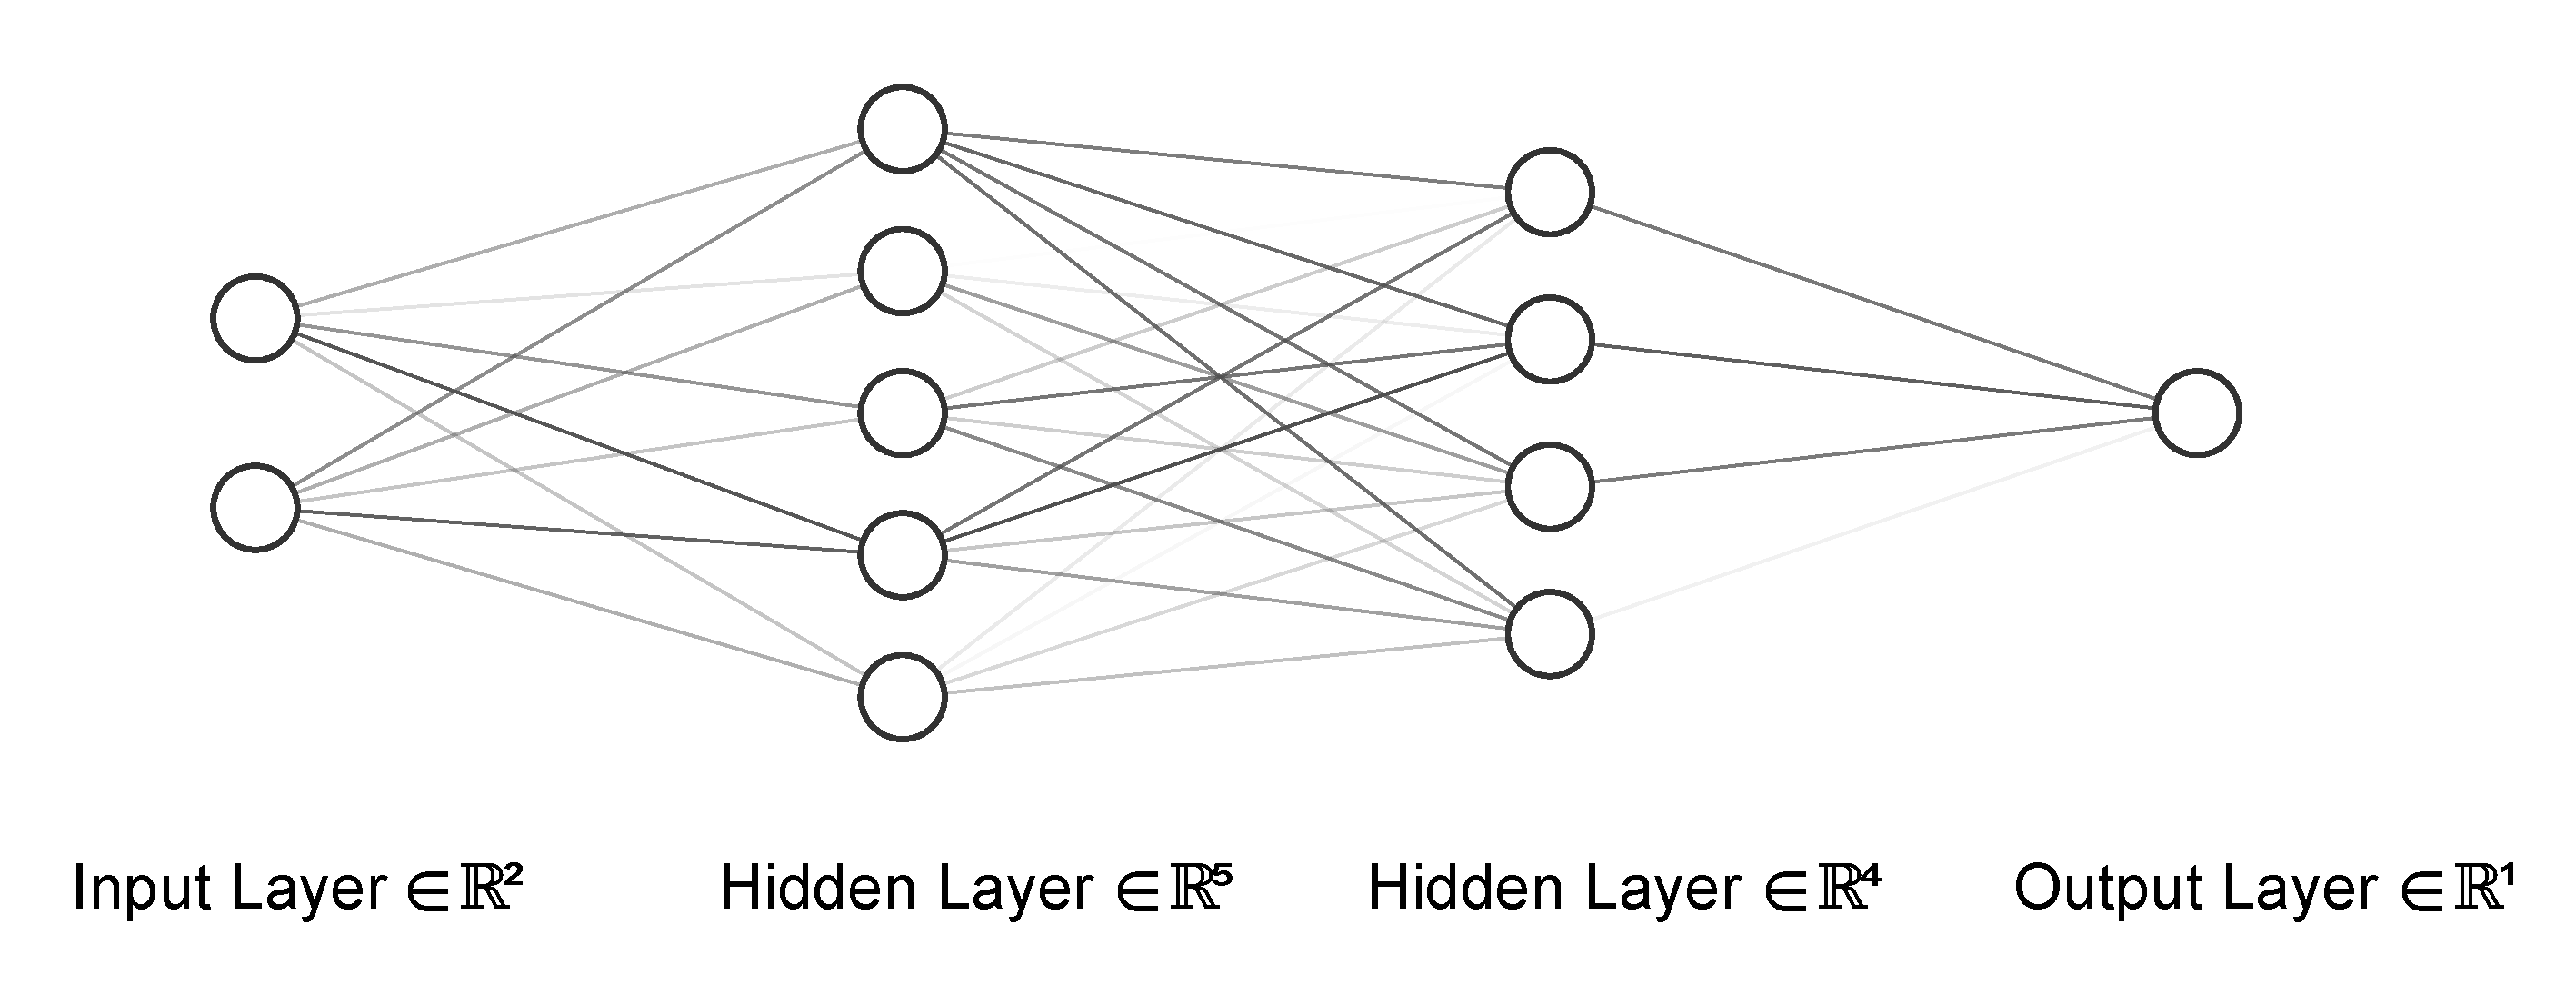
\includegraphics[width=1\linewidth]{images/simple_nn_architecture.pdf}
    % \includesvg{images/simple_nn_architecture.svg}
    \caption{An example trained fully connected neural network architecture with an input layer, two hidden layers, and an output layer. The weights are represented by the lines connecting the neurons, with opacity indicating the weights' strength.}
    \label{fig:simple-nn-architecture}
\end{figure}
Neural networks (NNs) represent a class of models that draw inspiration from the structural and functional characteristics of the biological brain. These models are designed to approximate complex functions by learning from data. A neural network consists of interconnected nodes, referred to as "neurons," which process input data to generate output. In the realm of supervised learning, neural networks are utilized to map input data—such as images—to desired outputs, for instance, restored or enhanced images.

\subsection{Basic Structure of Neural Networks}

% A typical neural network comprises several layers of neurons. The input layer serves as the first layer, receiving the input data, with each node corresponding to a specific feature of that data. Following the input layer, the network contains one or more hidden layers. These intermediate layers are crucial for computation and learning, as each neuron within a hidden layer computes a weighted sum of its inputs, applies a nonlinear activation function, and transmits the resulting value to the subsequent layer. Finally, the output layer produces the final output of the network based on the computations performed in the hidden layers.

% Connections between neurons are associated with weights that determine the strength and direction of the signals transmitted between them. The learning process of the network is achieved through the adjustment of these weights, which is accomplished via a method known as backpropagation. This process aims to minimize the error between the predicted output and the actual target by modifying the weights according to the gradient of the loss function.

\subsection{Activation Functions}

% To introduce non-linearity into the model, each neuron typically applies an activation function to the weighted sum of its inputs. Common activation functions include the sigmoid function, which maps input values to a range between 0 and 1, making it particularly useful in binary classification tasks. The Rectified Linear Unit (ReLU) sets negative inputs to zero while preserving positive inputs, and it is widely favored due to its simplicity and effectiveness in training deep networks. Additionally, the hyperbolic tangent (tanh) function maps input values to a range between -1 and 1, and it is often employed in the hidden layers of neural networks. The selection of an appropriate activation function significantly influences the network's performance and its ability to learn complex patterns within the data.

\subsection{Training Neural Networks}

% Training a neural network involves two primary phases: the forward pass and the backward pass. During the forward pass, the input data is propagated through the network, layer by layer, to generate an output. Following this, the backward pass occurs, in which the error—defined as the difference between the predicted output and the true output—is propagated back through the network using the gradient of the loss function. This step is crucial for updating the weights of the network.

% The objective of training is to minimize the loss function, which quantifies the discrepancy between the predicted output and the true output. Common loss functions include Mean Squared Error (MSE), which is often used in regression tasks, and Cross-Entropy, which is prevalent in classification tasks. The training process utilizes optimization algorithms, such as Stochastic Gradient Descent (SGD) or Adam, which iteratively adjust the network's weights to reduce the loss.

\subsection{Universal Approximation Theorem}

% A fundamental result in the theoretical framework of neural networks is the Universal Approximation Theorem. This theorem posits that a feedforward neural network, possessing at least one hidden layer and a sufficient number of neurons, can approximate any continuous function on a compact subset of \(\mathbb{R}^n\) to any desired degree of accuracy, provided that the network employs a non-linear activation function.


% The theorem can be formally articulated as follows: For any continuous function \(f: \mathbb{R}^n \to \mathbb{R}\) and for any \(\epsilon > 0\), there exists a feedforward neural network \(N\) with at least one hidden layer, a finite number of neurons, and an activation function (such as sigmoid or ReLU), such that for every \(x \in \mathbb{R}^n\), the inequality 

% $|f(x) - N(x)| < \epsilon$

% holds true. This result underscores the potential of neural networks; with an adequate number of neurons, they are capable of approximating complex, high-dimensional functions, independent of the underlying distribution of the data.

% The Universal Approximation Theorem carries significant implications for the field of machine learning. Primarily, it highlights the expressive power of neural networks, which, in theory, can approximate any function. This versatility renders them highly effective for a wide array of tasks, including image classification, restoration, and speech recognition. 

% While the theorem assures that a shallow network, possessing a single hidden layer, can approximate any function, practical applications often benefit from the utilization of deeper networks, which contain multiple hidden layers. Deeper networks typically require fewer neurons to achieve a comparable level of approximation and possess the capability to learn hierarchical representations of data. This characteristic is particularly advantageous in tasks involving images and language.

% Despite the theoretical capabilities outlined by the Universal Approximation Theorem, practical challenges persist in training these models effectively. Issues such as local minima, vanishing gradients, and overfitting can complicate the training process. Furthermore, the number of neurons necessary to achieve the desired accuracy may be prohibitively large, leading to substantial computational demands.

% In summary, the Universal Approximation Theorem emphasizes the considerable potential of neural networks to model intricate patterns. However, the practical success of a neural network is contingent upon careful design, tuning, and training of the model.



\section{Training}

If we generate images with overlapping subsets, the formed images are not independent, as the same events could be present in multiple images. A simple example would be to generate image an image with \num{e6} counts and other with twice as many counts, where the former is a subset of the latter. This is a limitation of the method, but it is a reasonable approximation for the purpose of this study.

\begin{figure}[h]
    \centering
    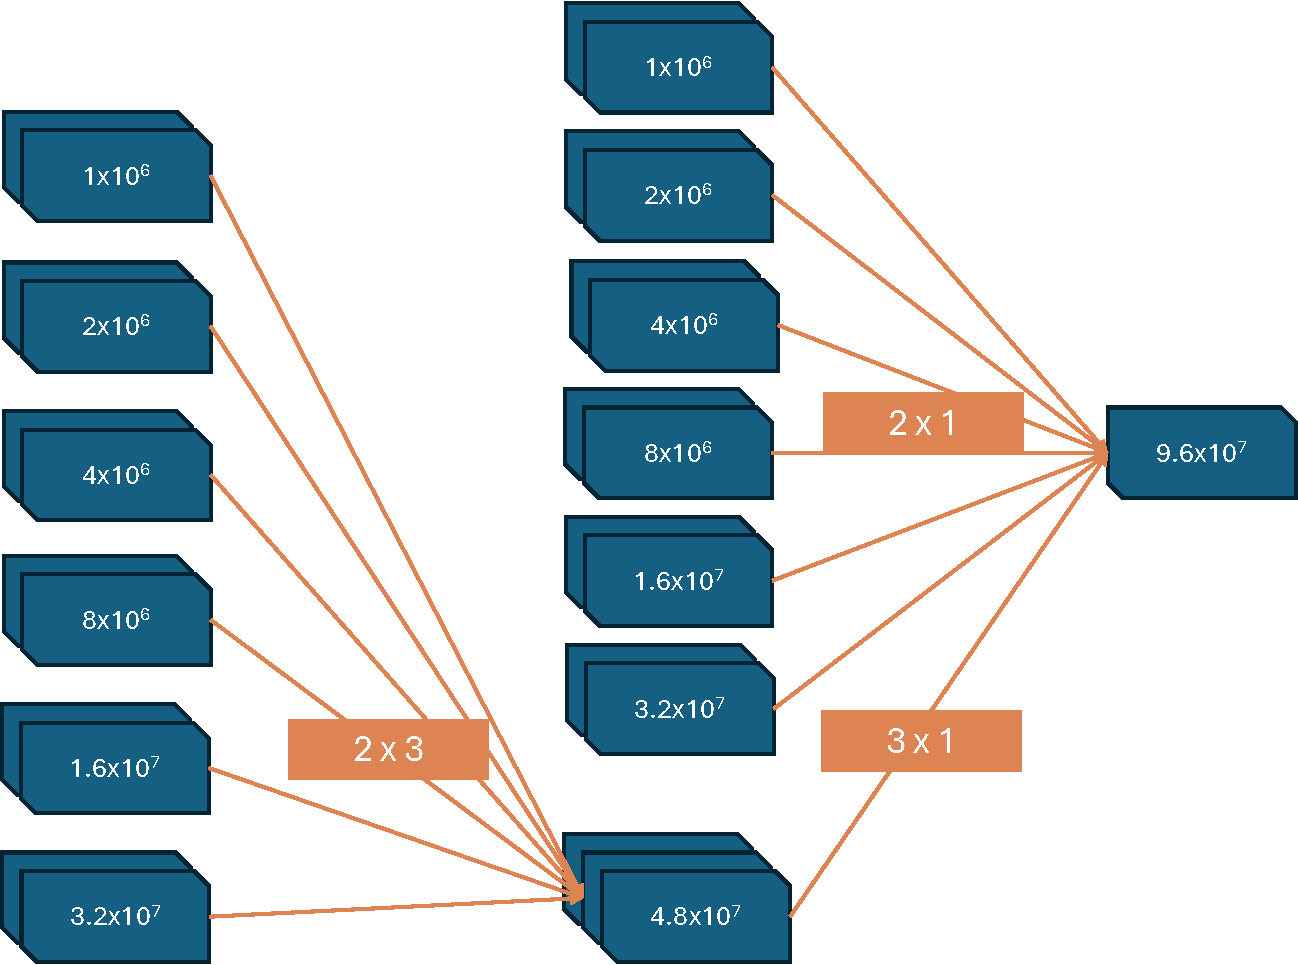
\includegraphics[width=1\linewidth]{images/training_flowchart.pdf}
    \caption{Flowchart illustrating the input-target dataset pairs used for neural network training, derived from subsets of the \gls{GrIr} dataset. A total of \num{34} unique noisy subsets are represented, with each dataset corresponding to one blue box in the chart. The different combinations shown in the chart generate \num{51} input-target pairs across various counts, including \numlist{1e6;2e6;4e6;8e6;1.6e7;3.2e7;4.8e7;9.6e7}. Notably, the \num{4.8e7} and \num{9.6e7} counts serve as the target datasets, with \num{9.6e7} additionally functioning as the target for the \num{4.8e7} datasets.}
    \label{fig:training-data}
\end{figure}

\begin{figure}[h]
    \centering
    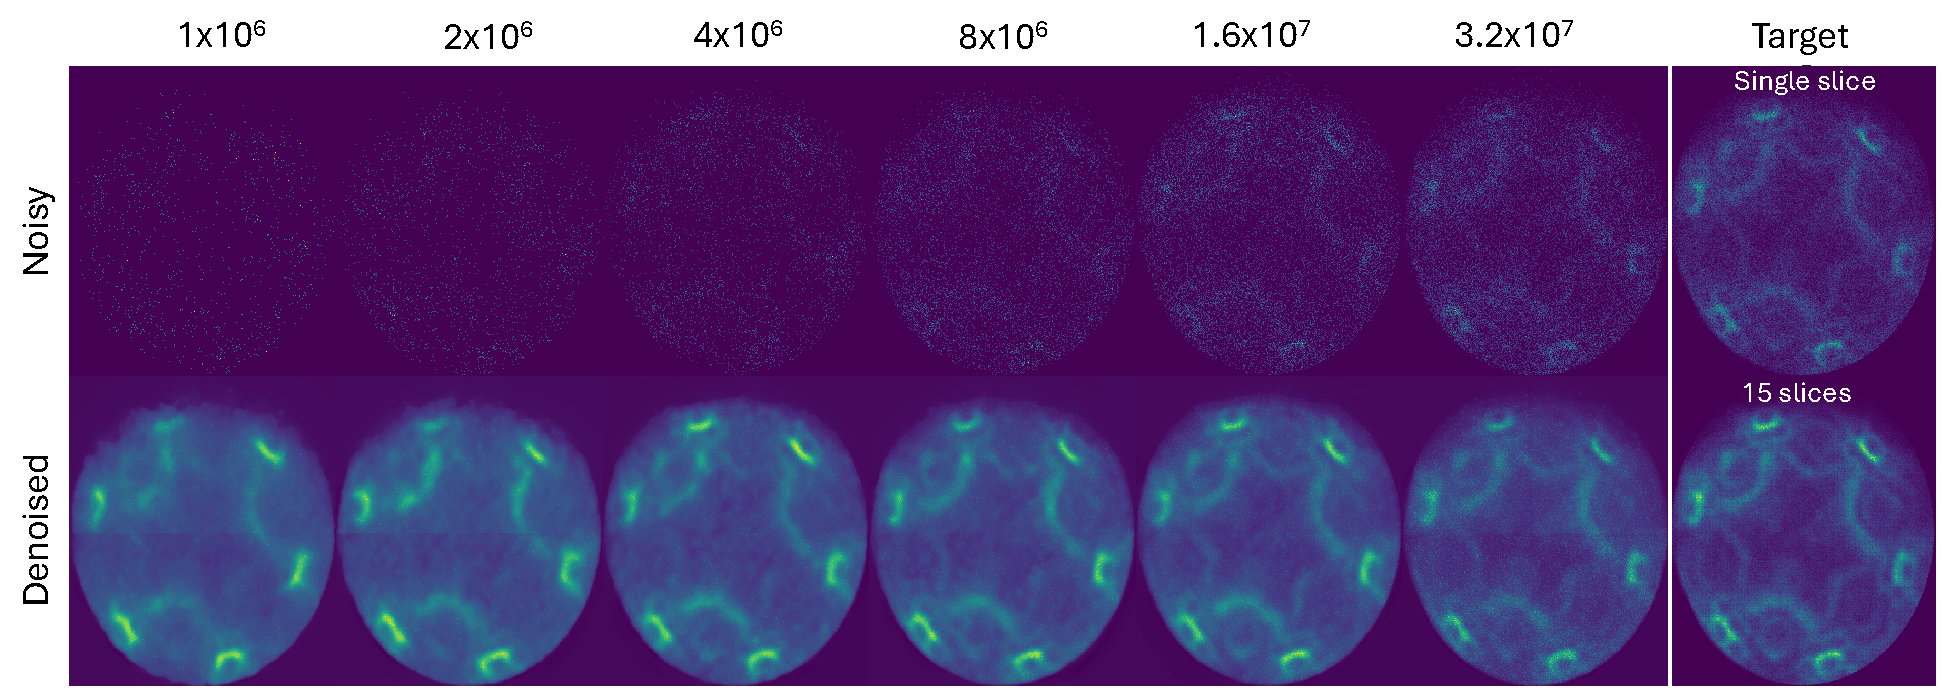
\includegraphics[width=1\linewidth]{images/images_noisy_denoised_with_target.pdf}
    \caption{Noisy and denoised \gls{ky}-\gls{kx} cuts with window size $w=1$ shown for \gls{GrIr} dataset. Each column corresponds to \numlist{1e6;2e6;4e6;8e6;1.6e7;3.2e7;1.86e8} counts, respectively; where the last column is the target image with $w=1$ in row 1 and $w=15$ in row 2. Below \num{8e6} counts, none of the features are discernible for noisy images, while the denoised images show clear features similar to the target.}
    \label{fig:images-noisy-denoised-training}
\end{figure}


\begin{figure}[h]
    \centering
    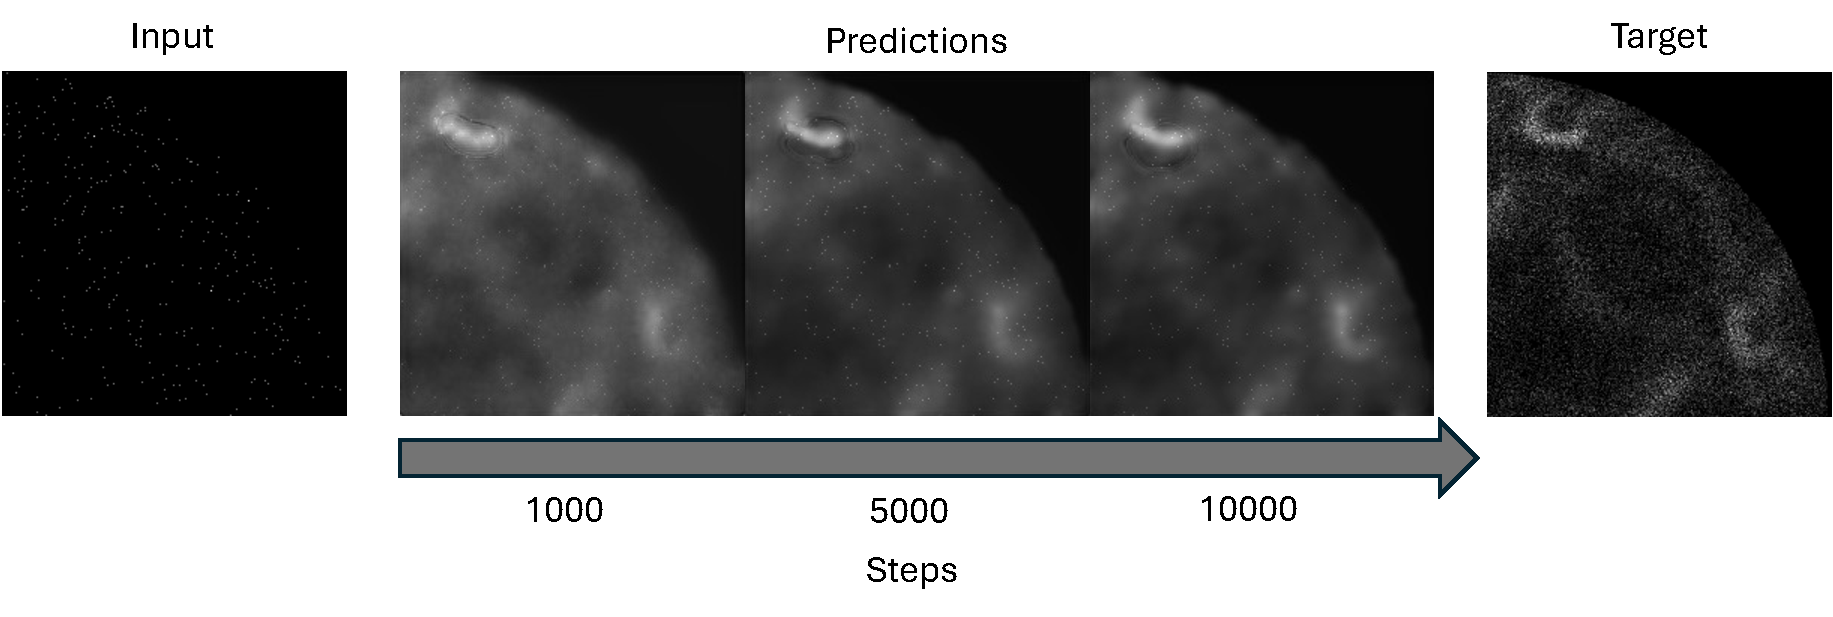
\includegraphics[width=1\linewidth]{images/training_progress_example2.pdf}
    \caption{}
    \label{fig:training-progress-example}
\end{figure}


\begin{figure}
    \centering

    \begin{subfigure}[b]{0.7\linewidth}
        \centering
        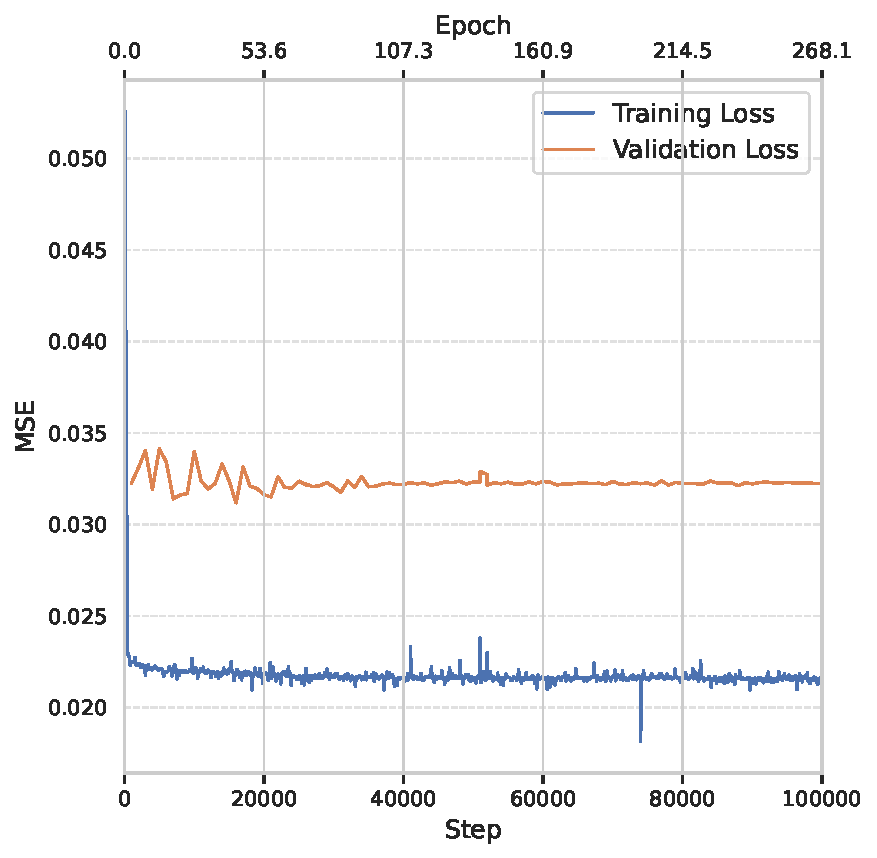
\includegraphics[width=1\linewidth]{images/loss_training_val.pdf}
        \caption{}
        \label{fig:loss-training-val}
    \end{subfigure}

    \begin{subfigure}[b]{0.7\linewidth}
        \centering
        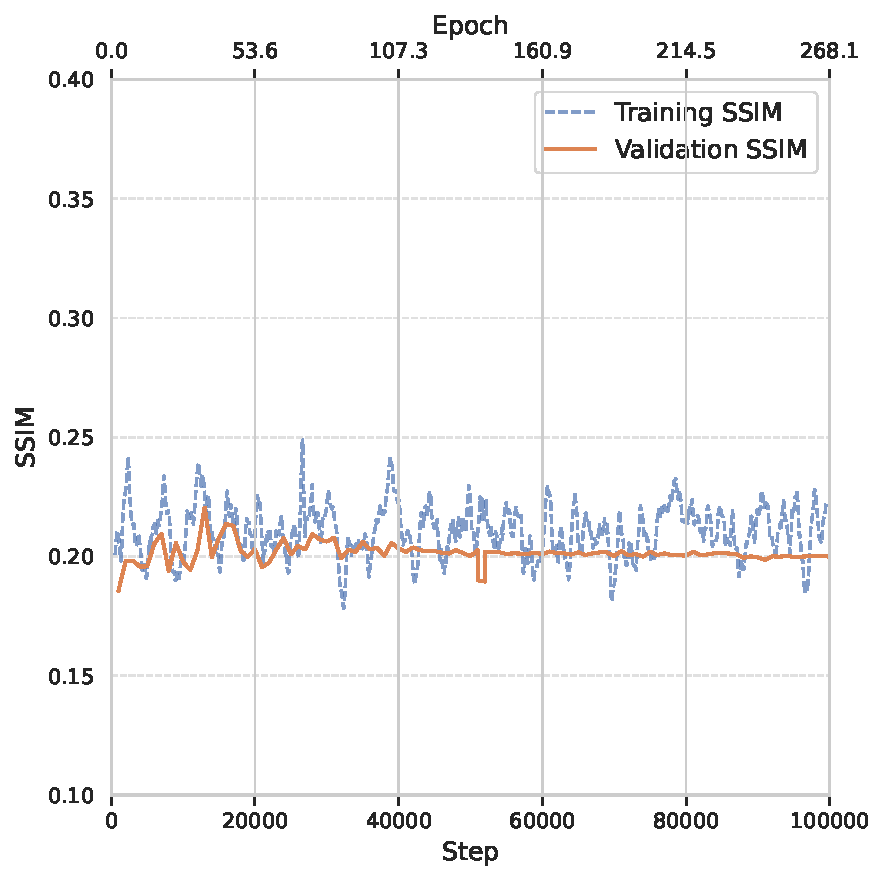
\includegraphics[width=1\linewidth]{images/ssim_training_val.pdf}
        \caption{}
        \label{fig:ssim-training-val}
    \end{subfigure}

    \caption{Training and validation loss and \gls{SSIM} scores for the neural network model trained on the \gls{GrIr} dataset.}
    \label{fig:loss-ssim-training-val}
\end{figure}

\section{Testing}
\begin{figure}[h]
    \centering
    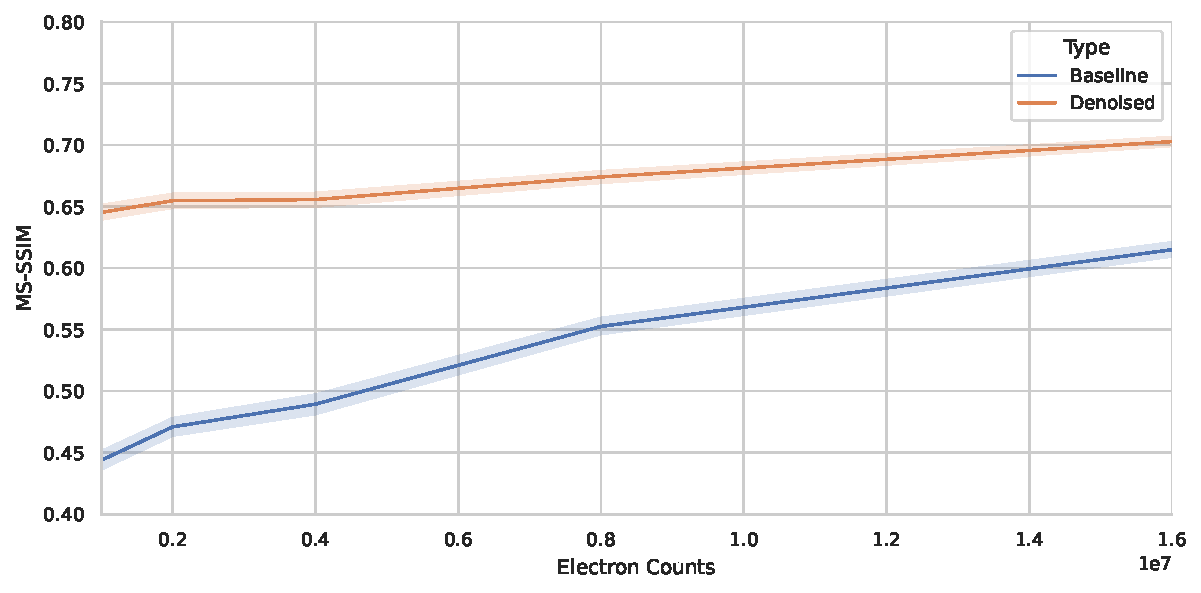
\includegraphics[width=1\linewidth]{images/nn_gdw_msssim.pdf}
    \caption{\num{1e6} counts take approximately \qty{11.5}{min} to acquire. \gls{GdW} dataset.}
    \label{fig:gdw-test-metirc}
\end{figure}


\begin{figure}
    \centering
    \begin{subfigure}[b]{1\linewidth}
        \centering
        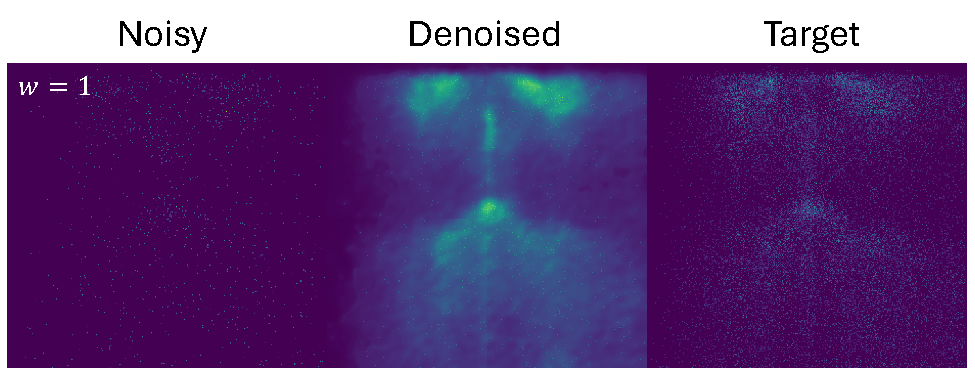
\includegraphics[width=1\linewidth]{images/nn_denoised_ex_w_1.pdf}
        \caption{}
        \label{fig:nn-denoised-ex-w-1}
    \end{subfigure}

    \begin{subfigure}[b]{1\linewidth}
        \centering
        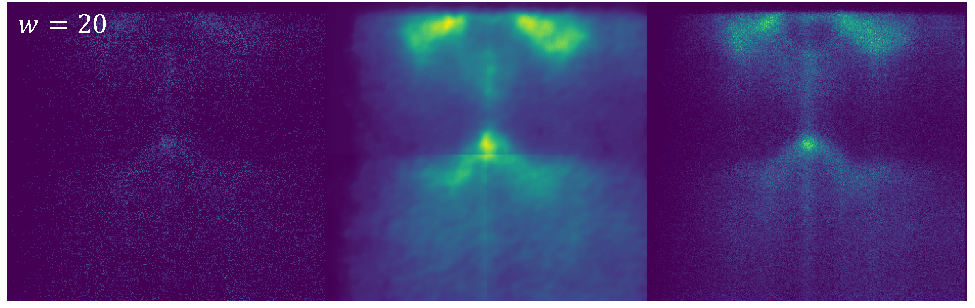
\includegraphics[width=1\linewidth]{images/nn_denoised_ex_w_20.pdf}
        \caption{\num{4e6} count dataset. The denoising performance leaves room for improvement, using the adjusted optimal $\sigma_{\text{o}}\approx0.4$.}
        \label{fig:nn-denoised-ex-w-20}
    \end{subfigure}
    \caption{}
    \label{fig:nn-denoised-ex-w}
\end{figure}

\begin{figure}
    \centering
    \begin{subfigure}[b]{1\linewidth}
        \centering
        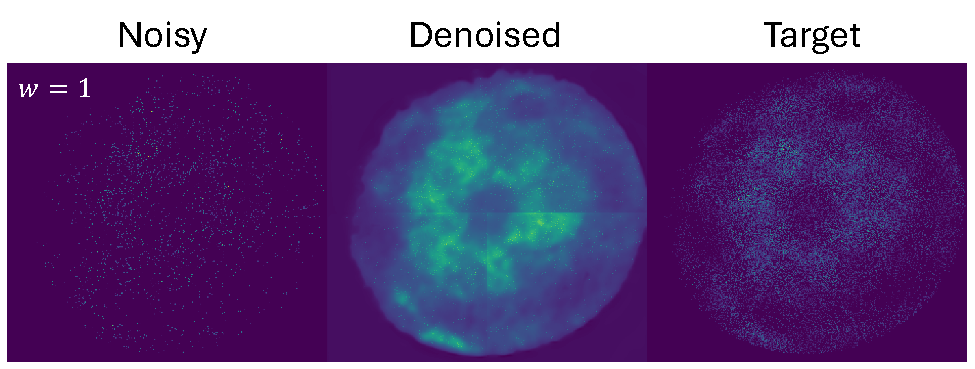
\includegraphics[width=1\linewidth]{images/nn_denoised_xy_w_1.pdf}
        \caption{}
        \label{fig:nn-denoised-xy-w-1}
    \end{subfigure}

    \begin{subfigure}[b]{1\linewidth}
        \centering
        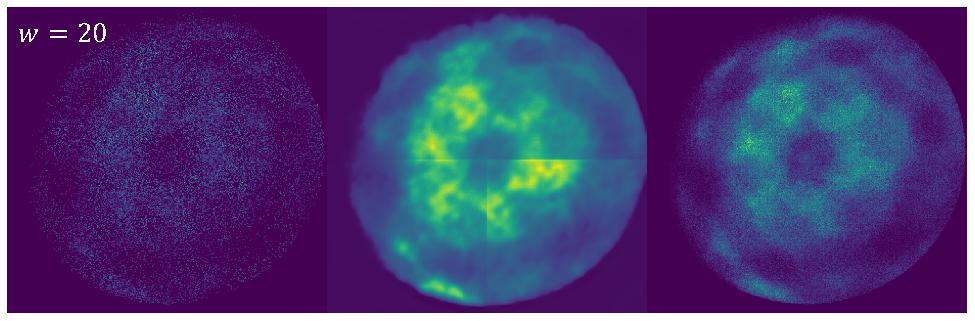
\includegraphics[width=1\linewidth]{images/nn_denoised_xy_w_20.pdf}
        \caption{}
        \label{fig:nn-denoised-xy-w-20}
    \end{subfigure}
    \caption{}
    \label{fig:nn-denoised-xy-w}
\end{figure}